\section{Experiments and Performance}
\label{experiments}

\subsection{Raytracing}

This section shows initial testing of the raytracer in Figures \ref{fig:firsttrace} and \ref{fig:secondtrace}. While the raytracer is plotting points in three dimensions, only a cross section of these plots is shown for clarity.

\begin{figure}
\centering
\begin{subfigure}{.5\textwidth}
  \centering
  \includegraphics[width=7cm]{out.png}
  \caption{Testing calculation of surface normals.}
  \label{fig:sub1}
\end{subfigure}%
\begin{subfigure}{.5\textwidth}
  \centering
  \includegraphics[width=7cm]{out2.png}
  \caption{Testing calculation of Snell's Law. An array of vertical rays generate these lines (not shown).}
  \label{fig:sub2}
\end{subfigure}
\label{fig:firsttrace}
\end{figure}

\begin{figure}
\centering
\begin{subfigure}{.5\textwidth}
  \centering
  \includegraphics[width=7cm]{out4.png}
  \caption{Testing multi surface refraction shows convergance of parallel rays.}
  \label{fig:sub3}
\end{subfigure}%
\begin{subfigure}{.5\textwidth}
  \centering
  \includegraphics[width=7cm]{out5.png}
  \caption{Testing the full lens system used for our simulations.}
  \label{fig:sub4}
\end{subfigure}
\label{fig:secondtrace}
\end{figure}


\subsection{Training and Regression}

We had limited time to perform experiments due to the late arrival of our dataset.  However, the tests that we did perform clearly show that our distributed logistic classifier scales well to achieve significant performance gains.  In addition to provable performance gains, we also observed Gustafson's Law in action in that the available parallelism significantly increases with our problem size.

For our initial tests, we ran two training sets through the classifier.  The first training set was small (283M) and the second set was larger (2.9G).  Our first goal was to observe the classification accuracy on of the classifier on the testing set.  Using the small training set, we were easily able to achieve 100\% accuracy.  This indicates that the amount of noise was insufficient and/or that there were not enough rays sampled to adequately obscure label partition boundaries.

Figures \ref{fig:small} \ref{fig:big} show performance gains for our initial tests.  We clearly see that while available parallelism levels out around 10 nodes with a student account on ACISS, the amount of available parallelism dramatically increases with our problem size.  The small dataset achieves a speedup of approximately 7 times relative to the serial execution while the larger dataset achieves roughly 9 times speed up.  This is an embarrassingly parallel problem with limited communication demands, so it is reassuring to see almost 10 times speedup with 10 times the computational power.  This implies that our implementation efficiently utilizes the parallel processing power to take advantage of available parallelism.

\begin{figure}[h]
\begin{center}
\includegraphics[scale=0.7]{small_metrics.png}
\caption{Performance gains for both data loading and iteration time on the small training set.}
\label{fig:small}
\end{center}
\end{figure}

\begin{figure}[h]
\begin{center}
\includegraphics[scale=0.7]{big_metrics.png}
\caption{Performance gains for both data loading and iteration time on the large training set.}
\label{fig:big}
\end{center}
\end{figure}

\subsection{Visualization}

Visualizations of both the simulated CCD images and the output of the classifier allow us to qualitatively compare our simulated system to what we expect to find in the actual experiment. The visualization in Figures \label{ccd2d} and \label{contours}  in were generated with Mathematica.

\begin{figure}
  \centering
  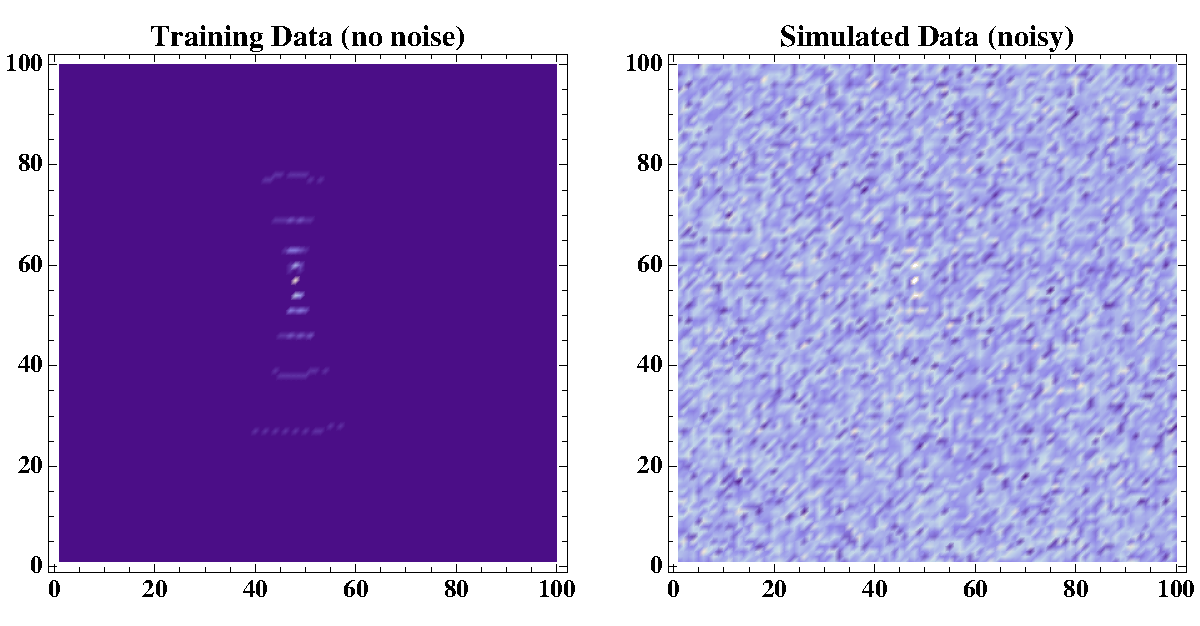
\includegraphics[scale=0.7]{ccd2d.png}
  \label{ccd2d}
  \caption{This shows a pair of simulated CCD images created by our raytracer. The left image is directly from the raytracer, while the right image has the addition of poissionian noise, which simulates the dark counts that are ordinarily found with CCD images. Images like the one on the left were used to train the classifier while images like on the right were used for testing the classification.}
\end{figure}

\begin{figure}
 \label{contours}
\centering
\begin{subfigure}{.5\textwidth}
  \centering
  \includegraphics[scale=.35]{2-5.pdf}
\end{subfigure}%
\begin{subfigure}{.5\textwidth}
  \centering
  \includegraphics[scale=.35]{4-3.pdf}
\end{subfigure}
\label{fig:test2}
\caption{These images are visualizations of the probability distribution output generated by our classifier, which marks the most likely locations for the atom to be positioned according to the classifier. The arrow marks where the atom actually was located before the rays were traced. All of the tests appear very similar to this image.}
\end{figure}
